\documentclass[t]{beamer}
\mode<presentation>

\usepackage{etex}

\usetheme{Madrid}
% other themes: Warsaw, AnnArbor, Antibes, Bergen, Berkeley, Berlin, Boadilla, boxes, CambridgeUS, Copenhagen, Darmstadt, default, Dresden, Frankfurt, Goettingen,
% Hannover, Ilmenau, JuanLesPins, Luebeck, Madrid, Maloe, Marburg, Montpellier, PaloAlto, Pittsburg, Rochester, Singapore, Szeged, classic

\setbeamertemplate{navigation symbols}{\insertslidenavigationsymbol}

\usecolortheme{dolphin}
%\usecolortheme{seagull}
% color themes: albatross, beaver, beetle, crane, default, dolphin, dov, fly, lily, orchid, rose, seagull, seahorse, sidebartab, structure, whale, wolverine

%\usefonttheme{serif}
% font themes: default, professionalfonts, serif, structurebold, structureitalicserif, structuresmallcapsserif

% pdf is displayed in full screen mode automatically
%\hypersetup{pdfpagemode=FullScreen}

%\AtBeginSection[]
%{
%  \begin{frame}<beamer>
%    \frametitle{Outline}
%    \tableofcontents[currentsection,currentsubsection]
%  \end{frame}
%}

% define your own colours:
\definecolor{Red}{rgb}{1,0,0}
\definecolor{Blue}{rgb}{0,0,1}
\definecolor{Green}{rgb}{0,1,0}
\definecolor{magenta}{rgb}{1,0,.6}
\definecolor{lightblue}{rgb}{0,.8,1}
\definecolor{lightpurple}{rgb}{.6,.4,1}
\definecolor{gold}{rgb}{.6,.5,0}
\definecolor{orange}{rgb}{1,0.4,0}
\definecolor{hotpink}{rgb}{1,0,0.5}
\definecolor{newcolor2}{rgb}{.5,.3,.5}
\definecolor{newcolor}{rgb}{0,.3,1}
\definecolor{newcolor3}{rgb}{1,0,.35}
\definecolor{darkgreen1}{rgb}{0, .35, 0}
\definecolor{darkgreen}{rgb}{0, .6, 0}
\definecolor{darkred}{rgb}{.75,0,0}

\xdefinecolor{olive}{cmyk}{0.64,0,0.95,0.4}
\xdefinecolor{purpleish}{cmyk}{0.75,0.75,0,0}

%\usepackage{beamerinnerthemerounded}
% inner themes include circles, default, inmargin, rectangles, rounded

%\usepackage{beamerouterthemesmoothbars}
% outer themes include default, infolines, miniframes, shadow, sidebar, smoothbars, smoothtree, split, tree

\useoutertheme[subsection=false]{smoothbars}

% to have the same footer on all slides
\setbeamertemplate{footline}[text line]{

\includegraphics[height=15pt]{sulogolong.eps}\hfill 
\raisebox{5pt}{Math 207:  Introduction to Statistics}\hfill 
\raisebox{5pt}{Chapter 12: The  Regression Line}\hfill
\raisebox{5pt}{\insertframenumber/\pageref{lastpage}}}
%\setbeamertemplate{footline}[text line]{} % or empty footer

% include packages
\usepackage{subfigure}
\usepackage{multicol}
\usepackage{amsmath}
\usepackage{epsfig}
\usepackage{graphicx}
\usepackage[all,knot]{xy}
\xyoption{arc}
\usepackage{url}
\usepackage{multimedia}
\usepackage{hyperref}
\usepackage{setspace}

\title{Math 207:  Statistics}
\subtitle{Chapter 12:  The  Regression Line}
\author{Ralph Wojtowicz}
\institute{Mathematics Department\\ Shenandoah University}
%\date{\scriptsize 6 February 2012}

\usepackage{pstricks,pst-grad,pst-func,pst-text,pst-node,multido,pst-plot,calc,pst-3dplot}

\newcommand{\BRACE}{
\begin{pspicture}(-3,-2.1)(3,1.1)
\psset{yunit=3,linewidth=0.02}
\psline(-3.5,0)(3.5,0)  
  \psline(-3,0)(-3,-0.04) \rput[t](-3,-0.07){\scriptsize -3\hphantom{-}}
  \psline(-2,0)(-2,-0.04) \rput[t](-2,-0.07){\scriptsize -2\hphantom{-}}
  \psline(-1,0)(-1,-0.04) \rput[t](-1,-0.07){\scriptsize -1\hphantom{-}}
  \psline(0,0)(0,-0.04)   \rput[t](0,-0.07){\scriptsize 0}
  \psline(1,0)(1,-0.04)   \rput[t](1,-0.07){\scriptsize 1}
  \psline(2,0)(2,-0.04)   \rput[t](2,-0.07){\scriptsize 2}
  \psline(3,0)(3,-0.04)   \rput[t](3,-0.07){\scriptsize 3}
  \rput[l](3.6,0){\scriptsize $x$}
\psline(0,0)(0,0.5)
  \psline(-0.12,0.5)(0,0.5)    \rput[r](-0.21,0.5){\scriptsize $0.5$}
  \psline(-0.12,0.25)(0,0.25)  \rput[r](-0.21,0.25){\scriptsize $0.25$}
\psGauss[linecolor=blue,linewidth=0.02,sigma=1,mue=0]{-3}{3}
\pnode(-1,-0.15){A}\pnode(1,-0.15){B}
\psbrace[braceWidth=0.02,braceWidthInner=5pt,braceWidthOuter=5pt](A)(B){\rput{90}(0.25,-0.05){\scriptsize 68\%}}
%
\pnode(-2,-0.15){C}\pnode(2,-0.15){D}
\psbrace[braceWidth=0.02,braceWidthInner=25pt,braceWidthOuter=5pt](C)(D){\rput{90}(0.25,-0.05){\scriptsize 95\%}}
%
\pnode(-3,-0.15){E}\pnode(3,-0.15){F}
\psbrace[braceWidth=0.02,braceWidthInner=45pt,braceWidthOuter=5pt](E)(F){\rput{90}(0.25,-0.1){\scriptsize 99.7\%}}
\end{pspicture}}

\begin{document}

%\frame[plain]{
%	\titlepage
%}


\begin{frame}[plain]
\definecolor{myblue}{rgb}{0,0,0.6}
\definecolor{grayA}{rgb}{0.95,0.95,0.95}
\definecolor{grayB}{rgb}{0.98,0.98,0.98}
\begin{center}

%\begin{pspicture}(0,0)(7,4.8)
\begin{pspicture}(-6,-7)(6,2)
\rput(0,-1.85){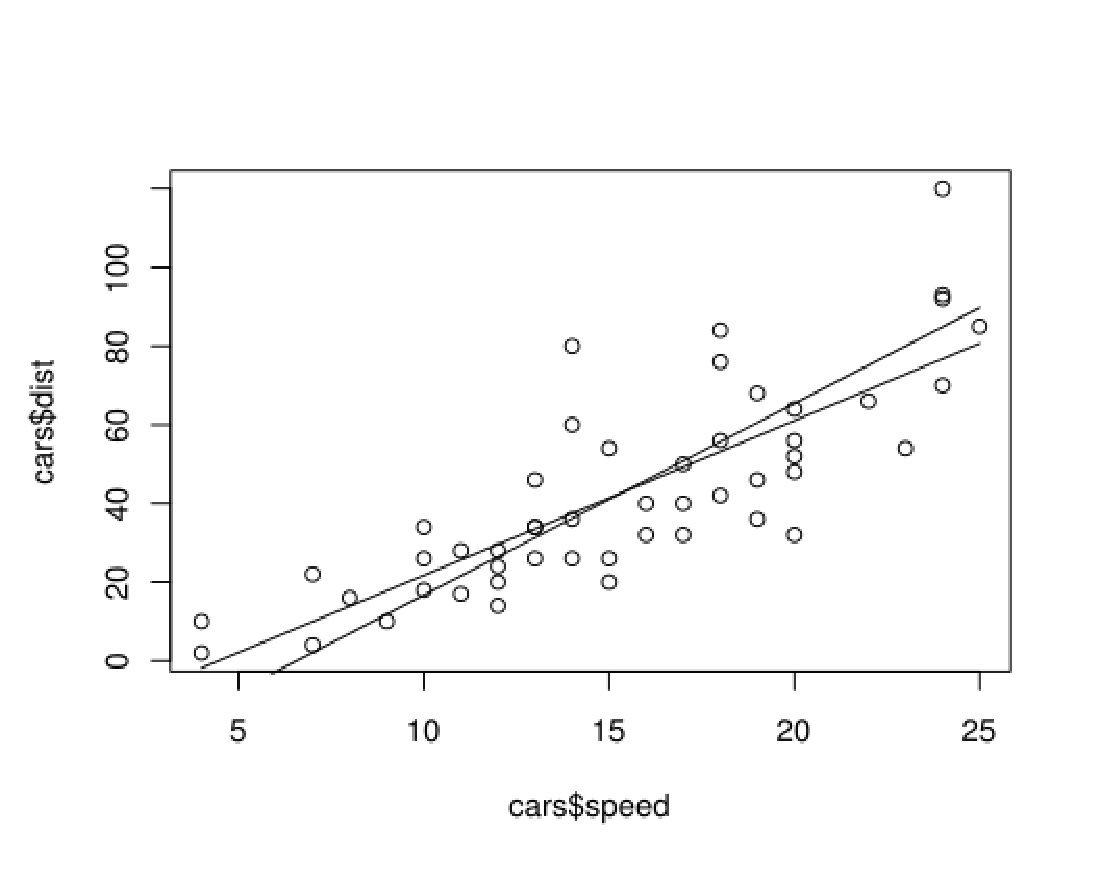
\includegraphics[height=4.2cm,bb=-0 -0 515 350,clip]{CarsRegression.eps}}
\psframe[linewidth=0.02,linecolor=gray](-6.2,-7)(6.2,2.2)
\psframe[linewidth=0.02,linecolor=gray](-6.15,-6.95)(6.15,2.15)
\rput(0,1.4){\color{myblue}\large Math 207:  Introduction to Statistics}
\rput(0,0.6){\color{myblue}Chapter 12:  The  Regression Line}
%\psframebox(0,0)(4,4)
\rput(0,-4.4){\scriptsize Dr.~Ralph Wojtowicz}
%\rput(0,-4.9){\scriptsize CME Department}
\rput(0,-5.6){
\includegraphics[height=2cm]{sulogolong.eps}}
%
%\rput(0,-6.5){\scriptsize 6 February 2012}
\end{pspicture}
\end{center}

\end{frame}

%\section[Outline]{}

\addtocounter{page}{-1}
\addtocounter{framenumber}{-1}

{\footnotesize
\frame{\tableofcontents}
}

\section{Regression Line}
\subsection{The Regression Line}
\begin{frame}[t]\frametitle{The Regression Line}

{\footnotesize
\begin{itemize}
\item For a given value of $x$, 
  \begin{itemize}
  \item \footnotesize the regression line estimates the {\color{darkgreen}average value for $y$} 
  \item \footnotesize the point on the line is the {\color{darkgreen}predicted $y$ for an individual}
  \end{itemize}
\item For each increase of one SD in $x$, there is an increase of  $r$ SDs in $y$.
%\item The equation for the regression line is: % (where $r=\mbox{the correlation
\end{itemize}

\begin{center}
\begin{pspicture}(-5,0)(4.0,2.5)
  \psset{xunit=0.9,yunit=0.9}
  \rput(-3.5,1.25){$\displaystyle (y-\mbox{mean}_y) = {\color{blue}r\,\frac{\mbox{SD}_y}{\mbox{SD}_x}}\,(x-\mbox{mean}_x)$}
\psline{->}(0,0)(5,0)
\psline{->}(0,0)(0,3)
\psdot(1,1)
\psline[linewidth=0.02](1,1)(4,1)(4,2.5)
\psline[linewidth=0.02,linecolor=blue](1,1)(4,2.5)
\rput[b](1.4,2.25){\footnotesize $(\mbox{mean}_x, \mbox{mean}_y)$}
   \psline[linewidth=0.02]{->}(1.4,2.2)(1.02,1.1)
\rput[t](2.5,0.9){\footnotesize $\mbox{SD}_x$}
\rput[l](4.1,1.75){\footnotesize $r\,\mbox{SD}_y$}
\end{pspicture}\vspace{-10pt}
\end{center}

\begin{itemize}
\item The regression line is the line through the data that minimizes the RMS error.
\item $\mbox{RMS}_{\mbox{\scriptsize reg}} = \mbox{SD}_y\,\sqrt{1-r^2}$.
\item In vertical strips, the $y$ values approximately have a normal distribution with center
   on the line and with $\mbox{SD}=\mbox{RMS}_{\mbox{\scriptsize reg}}$.
\end{itemize}
}
\end{frame}

\section{Correlation}
\subsection{Correlation Coefficient}
\begin{frame}[t]\frametitle{The Correlation Coefficient}
{\small
\begin{itemize}
\item Given lists $x_1$, $\dots$, $x_n$ and $y_1$, $\dots$, $y_n$, the correlation
  coefficient:
  \begin{itemize} 
     \item Is a measure of linear association between the lists
     \item Is a measure of the clustering of the $(x_i, y_i)$ points around a line
     \item Is a number between $-1$ and $1$
     \item Is defined by:\vspace{-10pt}
   \end{itemize}
\end{itemize}
\begin{align*}
r &=\frac{1}{n}\,\sum_{i=1}^n\,\left(\frac{x_i - \mbox{mean}_x}{\mbox{SD}_x}\right)\,
  \left(\frac{y_i - \mbox{mean}_y}{\mbox{SD}_y}\right)\\
  &= \mbox{average of the $x$ and $y$ values measured in standard units}\vspace{-20pt}
\end{align*}\vspace{-15pt}
\begin{itemize}
\item A positive correlation means that the cloud of $(x_i, y_i)$ points slopes up
\item A negative correlation means that the cloud of $(x_i, y_i)$ points slopes down
\end{itemize}

}
\end{frame}

\subsection{Magnitude}
\begin{frame}
\frametitle{Sign and Magnitude of the Correlation Coefficient}

\begin{center}
\begin{pspicture}(0,0)(10,7)
%\psframe(0,0)(10,6)
\psline[linewidth=0.1,linecolor=purple]{<->}(0,6.5)(10,6.5)
\psline(5,6.7)(5,6.3)\rput(5,6.9){0.0}
\psline(0,6.7)(0,6.3)\rput(0,6.9){-1.0}
\psline(10,6.7)(10,6.3)\rput(10,6.9){1.0}
%
\rput(9,3){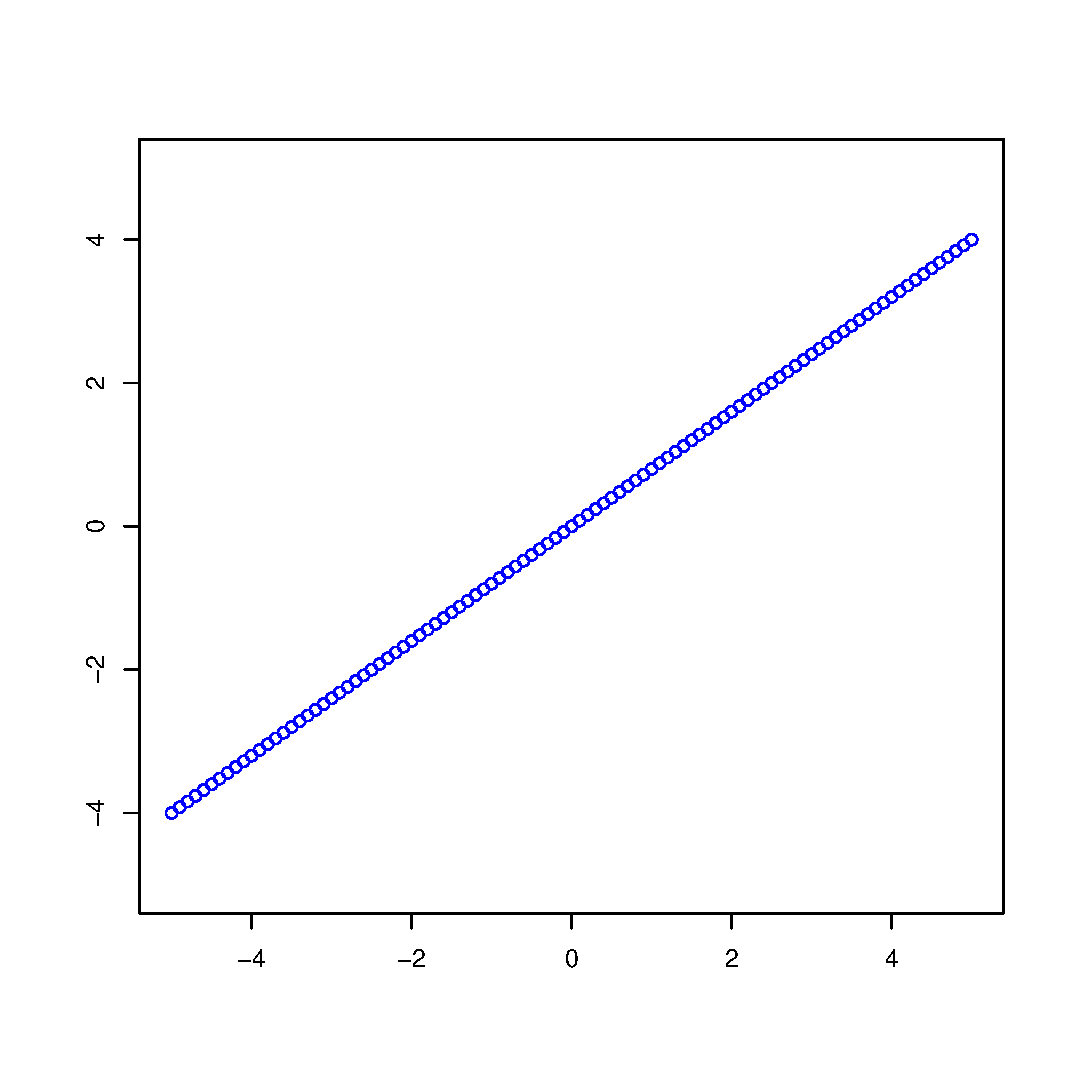
\includegraphics[height=1in]{cor1.eps}}    \rput(9,3.6){\footnotesize $r=1$}
\rput(7,1){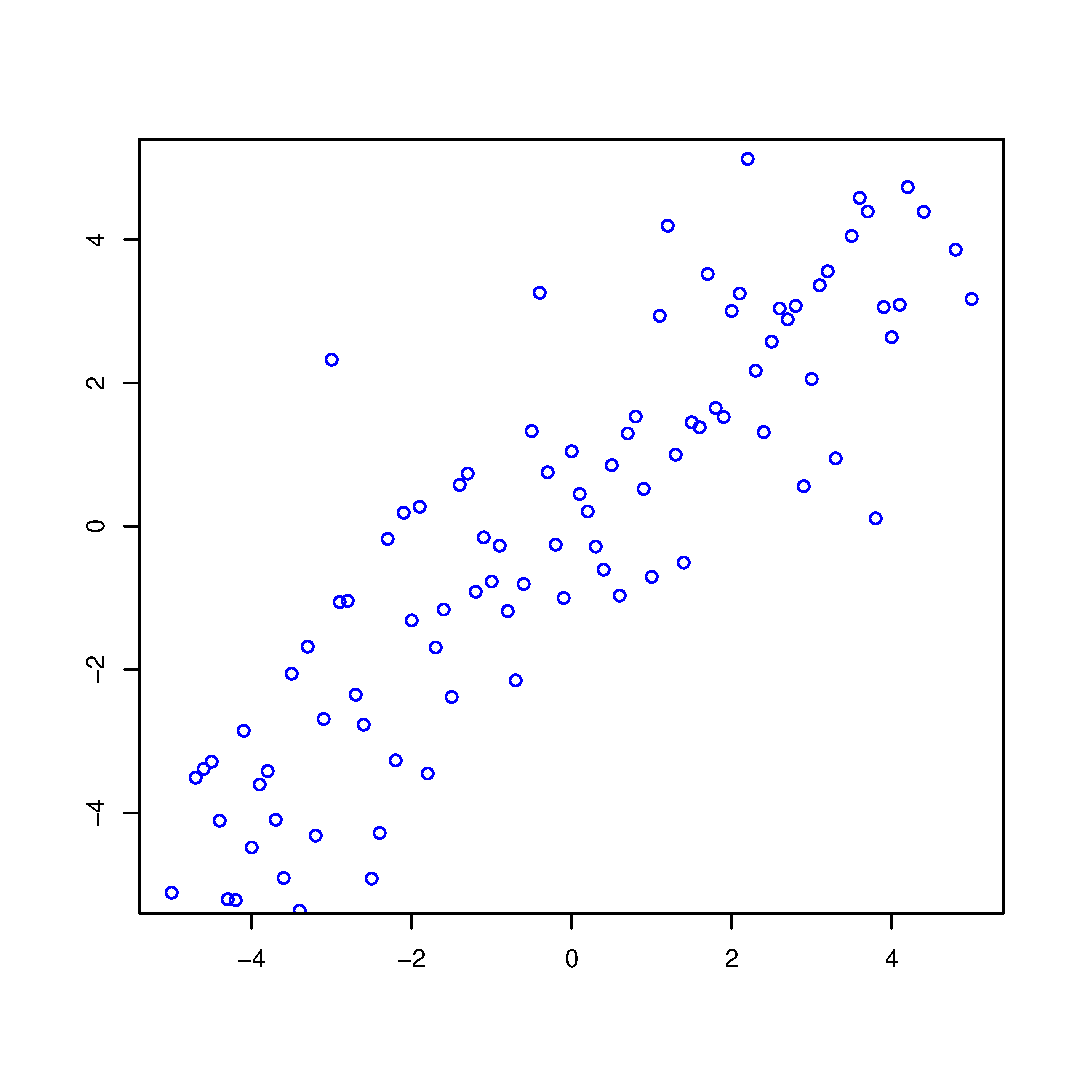
\includegraphics[height=1in]{cor_p9.eps}}  \rput(7,2.3){\footnotesize $r=0.9$}
\rput(6,5){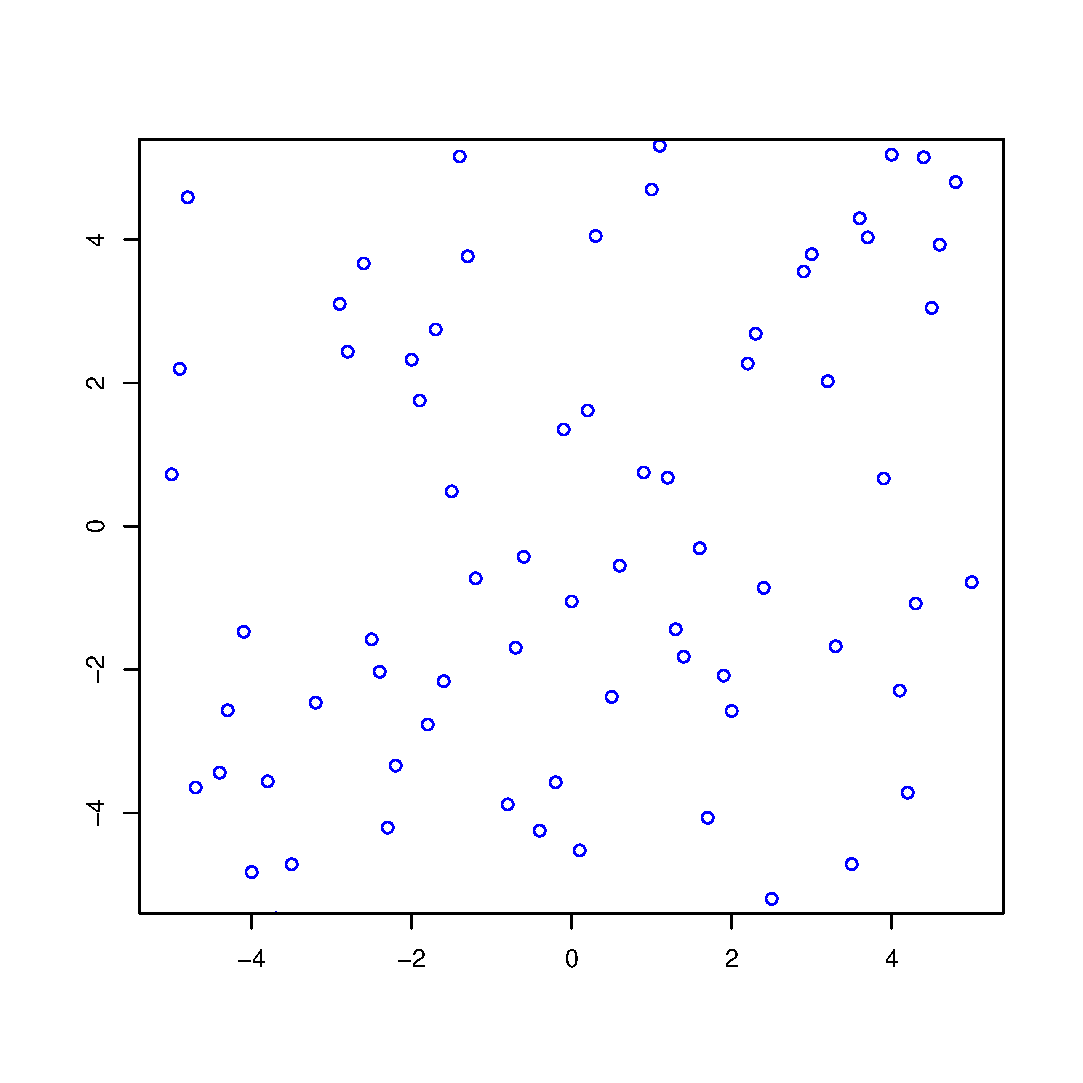
\includegraphics[height=1in]{cor_p4.eps}}  \rput(6,3.7){\footnotesize $r=0.4$}
%
\rput(4,1){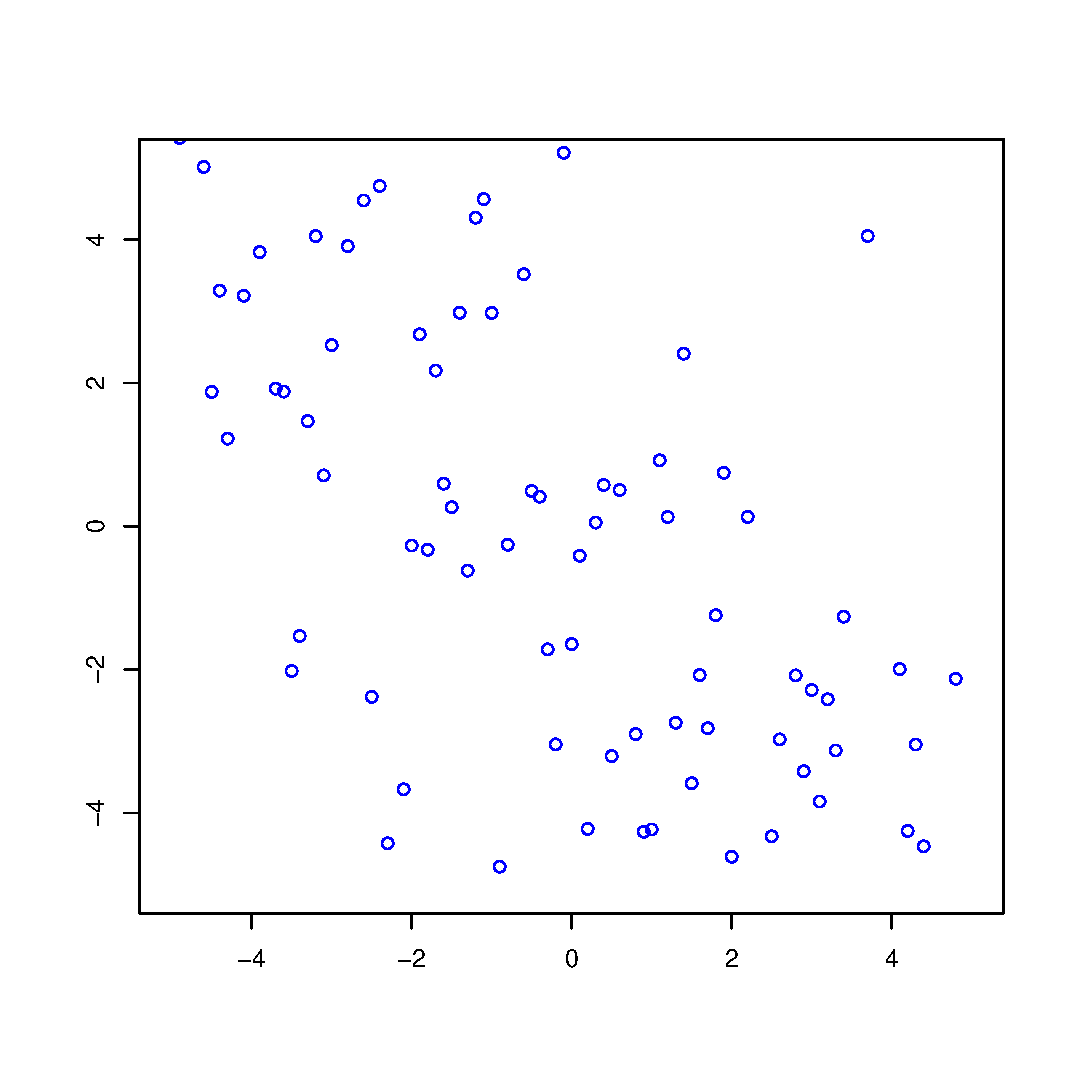
\includegraphics[height=1in]{cor_neg_p7.eps}} \rput(4,2.3){\footnotesize $r=-0.7$}
\rput(3,5){\includegraphics[height=1in]{cor_neg_p9.eps}} \rput(3.2,3.7){\footnotesize $r=-0.9$}
\rput(1,3){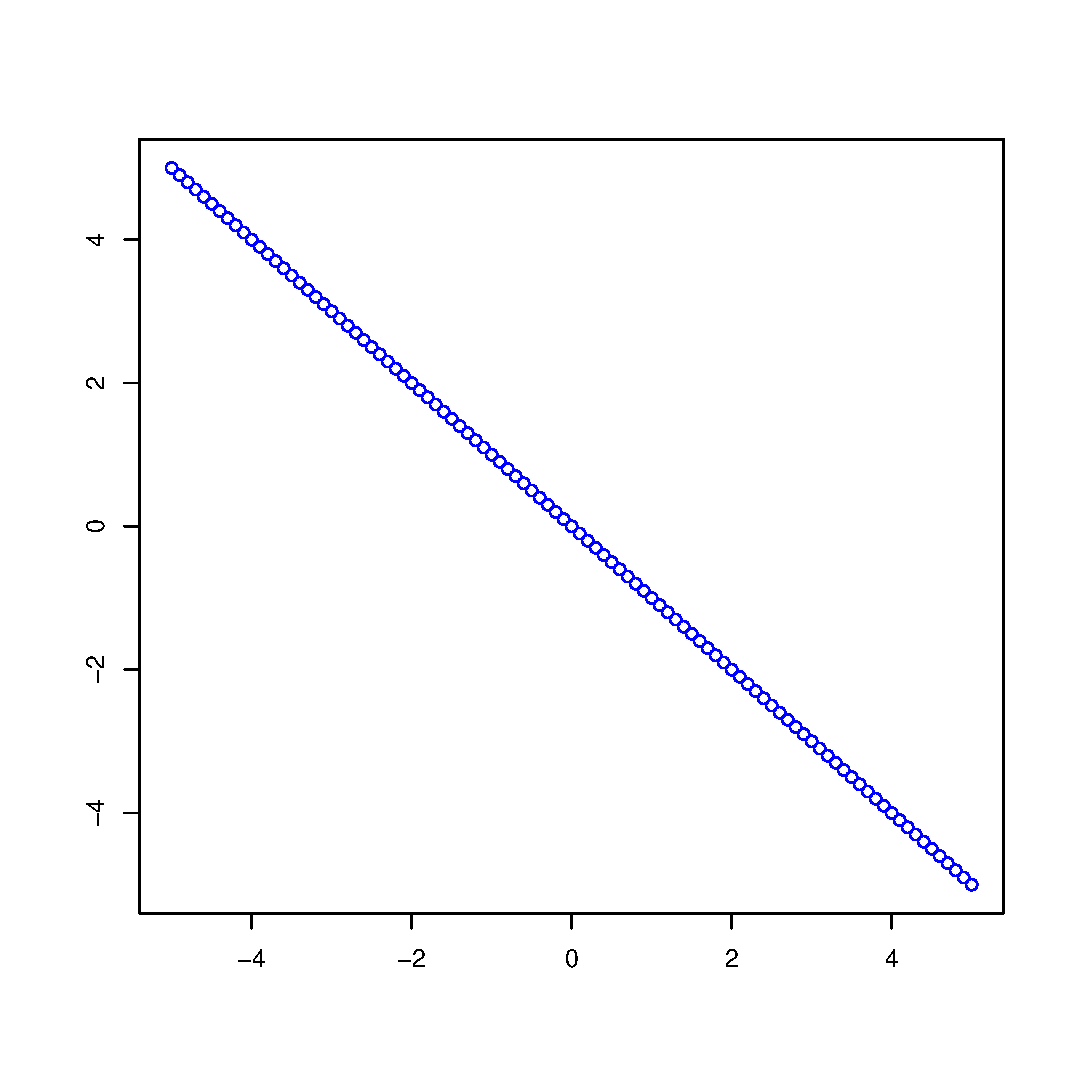
\includegraphics[height=1in]{cor_neg1.eps}} \rput(1,3.6){\footnotesize $r=-1$}
\end{pspicture}
\end{center}

\end{frame}

\section{Example}
\begin{frame}
\frametitle{Example}

\scriptsize

See Exercise 9 on page 215.   
\begin{center}
{\setlength{\tabcolsep}{2pt}\begin{tabular}{rclcrclcc}
average income & $\approx$ & \$90,000, & \hspace{5pt} & SD & $\approx$ & \$45,000,\\
average IQ & $\approx$ & 100, & \hspace{5pt} & SD & $\approx$ & 15, &
   \hspace{10pt} $r\approx 0.50$\\[-8pt]
\end{tabular}}
\end{center}

\begin{itemize}
\item<2-> Find the regression line for predicting IQ from income.\vspace{-3pt}
\[(y - 100) = 0.5\,\frac{15}{45,000}\,(x - 90,000)\hspace{10pt} \mbox{which is }\hspace{10pt}
  {\color{blue}(y - 100) = 0.000167\,(x - 90,000)}\]
\item<3-> Predict  IQ of an individual who makes \$120,000.  Put a plus or minus on your estimate.\\
  $y = 100 + 0.000167\,(120,000 - 90,000) \approx {\color{blue}105}$\\[3pt]
  The $\pm$ is $\mbox{RMS}_{\mbox{\scriptsize reg}} = \mbox{SD}_y\,\sqrt{1-r^2} = 15\sqrt{1-0.5^2}\approx 
   {\color{blue}13}$.\vspace{2pt}
\item<4-> About 95\% of the individuals who made \$120,000 had IQs in what range?
{\color{blue}  $105\pm 2\cdot 13$}
\item<5->  Find the regression line for predicting income from IQ.\vspace{-5pt}
\[(y - 90,000) = 0.5\,\frac{45,000}{15}\,(x - 100)\hspace{7pt} \mbox{which is }\hspace{7pt}
  {\color{blue}(y - 90,000) = 1500\,(x - 100)}\vspace{-3pt}\]
\item<6-> Predict the income of an individual whose IQ is 120.  Put a plus or minus on your estimate.\\[3pt]
  $y = 90,000 + 1500\,(120 - 100) = {\color{blue}120,000}$\\[3pt]
  The $\pm$ is $\mbox{RMS}_{\mbox{\scriptsize reg}} = \mbox{SD}_y\,\sqrt{1-r^2} = 45,000\sqrt{1-0.5^2}\approx 
   {\color{blue}\$39,000}$.
\end{itemize}
\label{lastpage}
\end{frame}

\end{document}

\begin{frame}
\frametitle{Title}


\end{frame}

\end{document}
